
\documentclass[11pt, a4paper]{book}
\usepackage[french]{babel}
\usepackage[utf8]{inputenc}
\usepackage{answers}

\usepackage{hyperref}
\usepackage{multicol}

\usepackage[table,xcdraw]{xcolor}
\usepackage{listings}
\definecolor{ForestGreen}{RGB}{34,139,34}


\usepackage{enumitem}

\AtBeginDocument{\def\labelitemi{$\bullet$}}


\newcommand{\py}{\lstinline{Python} }


\definecolor{backcolour}{rgb}{0.95,0.95,0.92}

\lstset{%
	language         = Python,
	backgroundcolor  = \color{backcolour},
	basicstyle       = \ttfamily, % \upshape\ttfamily,
	keywordstyle     = \bfseries\color{blue}, %\bfseries,
	stringstyle      = \color{magenta},
	commentstyle     = \color{ForestGreen},
	alsoletter = > ,
	morekeywords = {>>>,as,assert,False,None, nonlocal,True, with,yield , <<, >>, :},
	showstringspaces = false,
	numbers=left,
	stepnumber=1,
	literate={à}{{\`{a}}}1 {é}{{\'e}}1 {è}{{\`{e}}}1 {ê}{{\^{e}}}1 {Ê}{{\^{E}}}1 {î}{{\^i}}1 {ô}{{\^{o}}}1 {ç}{{\c{c}}}1 {Ç}{{\c{C}}}1
}

\newcommand{\itemb}[1]{\item \textbf{#1}}

\usepackage{fancyhdr}  %package pour en-tetes et pied de pages
\usepackage{sectsty} % Permet de faire des modifications de police dans diverses sections des "headings" (cf. modif presentation de la page)
\pagestyle{fancy}       %Style pour en-tetes et pieds de pages
\fancyhead[CO,CE]{\sc Série 1\hspace{0.5mm}}
\fancyhead[RO,LE]{Collège Sismondi}  % LaTeX/TEX define \strut to be an invisible box of width zero that extends just enough above and below the baseline. Cela permet d'augementer légèrement la taille en bas de la box de manière à ce qu'elle soit collée à la ligne.
\fancyhead[LO,RE]{\small\ \textsl{1\textsuperscript{ère} année - DO Informatique}}
\fancyfoot[RO,LE]{2021 - 2022}
\fancyfoot[LO,RE]{\small }
\fancyfoot[CO,CE]{\thepage}

\fancyhfoffset[l]{1.2cm} % le "l" en paramètre permet d'indiquer qu'on ne veut modifier que la marge à gauche.
\renewcommand{\headrule}{{%
		\hrule \headwidth \headrulewidth \vskip-\headrulewidth}}
\renewcommand\footrulewidth{\headrulewidth}
\renewcommand{\footrule}{{%
		\vskip-\footruleskip\vskip-\footrulewidth
		\hrule \headwidth \footrulewidth\vskip\footruleskip}}

\usepackage{tikz}
%-------------------------------------------------------------------------------
%---- Eclairage : en encadré sur fond jaune avec symbôle "ampoule" à gauche ----
%-------------------------------------------------------------------------------
\definecolor{coleclairage}{RGB}{255 , 221 , 156}
\definecolor{contoureclairage}{RGB}{255 , 192 , 0}
\newenvironment{eclairage}
{
	\begin{center}%
		\begin{tikzpicture}%
			\node[rectangle, draw=contoureclairage, top color=coleclairage!50, bottom color=coleclairage!140, rounded corners=5pt, inner xsep=5pt, inner ysep=6pt, outer ysep=10pt]\bgroup                     
			\begin{minipage}{0.98\linewidth}
				\begin{minipage}{0.08\linewidth}\centerline{
\includegraphics[scale=1]{Symbole_eclairage.png}}\end{minipage}
				\begin{minipage}{0.89\linewidth}\itshape\footnotesize
				}
				{                		
				\end{minipage}
			\end{minipage}\egroup;%
		\end{tikzpicture}%
	\end{center}%
}

%-------------------------------------------------------------------------------
%---- apprendre : en encadré sur fond jaune avec symbôle "ampoule" à gauche ----
%-------------------------------------------------------------------------------
\definecolor{colapprendre}{RGB}{50,205,50}
\definecolor{contourapprendre}{RGB}{34,139,34}
\newenvironment{apprendre}
{
	\begin{center}%
		\begin{tikzpicture}%
			\node[rectangle, draw=contourapprendre, top color=colapprendre!10, bottom color=colapprendre!50, rounded corners=5pt, inner xsep=5pt, inner ysep=6pt, outer ysep=10pt]\bgroup                     
			\begin{minipage}{0.98\linewidth}
				\begin{minipage}{0.08\linewidth}\centerline{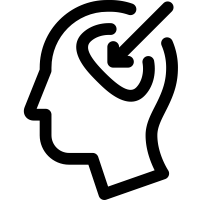
\includegraphics[width=30px]{Symbole_learn.png}}\end{minipage}
				\begin{minipage}{0.89\linewidth}\itshape\footnotesize
				}
				{                		
				\end{minipage}
			\end{minipage}\egroup;%
		\end{tikzpicture}%
	\end{center}%
}

\definecolor{colimportant}{RGB}{247 , 189 , 164}
\definecolor{contourimportant}{RGB}{237 , 125 , 49}
\newenvironment{important}
{
	\begin{center}%
		\begin{tikzpicture}%
			\node[rectangle, draw=contourimportant, top color=colimportant!50, bottom color=colimportant!140, rounded corners=5pt, inner xsep=5pt, inner ysep=6pt, outer ysep=10pt]\bgroup                     
			\begin{minipage}{0.08\linewidth}\centerline{
\includegraphics[scale=0.8]{Symbole_attention.png}}\end{minipage}
			\begin{minipage}{0.89\linewidth}
			}
			{                		
			\end{minipage}\egroup;
		\end{tikzpicture}%
	\end{center}%
}

%-----------------------------------------------------------------
%---- Modification présentation de la page: marges de la page ----
%-----------------------------------------------------------------
%\addtolength{\hoffset}{-1in}              % 1
%\addtolength{\voffset}{-1in}              % 2
\addtolength{\oddsidemargin}{-0.1 in} % 3
\addtolength{\evensidemargin}{-1in} % 3
\addtolength{\topmargin}{-1in}       % 4
\addtolength{\headheight}{6pt}       % 5
%\addtolength{\headsep}{-0.2cm}           % 6
\setlength{\textheight}{26cm}    % 7
\setlength{\textwidth}{16.5cm}      % 8
\addtolength{\marginparsep}{0pt}      % 9
\setlength{\marginparwidth}{0pt}   % 10
\addtolength{\footskip}{-1mm}           %11

\setlength{\parindent}{0em}% pas d'indentation


% Customiser le nom des sections
\usepackage{titlesec}
\titleformat{\section}[hang]{\Large \bfseries}{Série \thesection:\ }{0pt}{}

\renewcommand{\familydefault}{\sfdefault} % pour avoir des polices san serif

\newtheorem{Exc}{Exercice}
\Newassociation{correction}{Soln}{mycor}
\renewcommand{\Solnlabel}[1]{\bfseries Ex #1 }
\def\exo#1{%
	\futurelet\testchar\MaybeOptArgmyexoo}
\def\MaybeOptArgmyexoo{
	\ifx[\testchar \let\next\OptArgmyexoo
	\else \let\next\NoOptArgmyexoo \fi \next}
\def\OptArgmyexoo[#1]{%
	\begin{Exc}[#1]\normalfont}
	\def\NoOptArgmyexoo{%
		\begin{Exc}\normalfont}
		\newcommand{\finexo}{\end{Exc} \vspace{3mm}}
	\newcommand{\flag}[1]{}
	\newcommand{\entete}[1]

\newcommand{\getexocompteur}{{\the\numexpr \arabic{Exc}  \relax}}	
	
\newcommand{\eexo}{\vspace{5mm}} % espace pour séparer les exercices
\pgfplotsset{compat=1.17}
\begin{document}

\setcounter{chapter}{8}
\chapter{Programmation - Chaînes de caractères}
\section{Introduction}


Les chaînes de caractères (type \texttt{str)}  en Python sont des séquences de caractères qui peuvent être utilisées pour stocker des textes. Les chaînes de caractères sont définies entre apostrophes ('),  guillemets simples ("), ou  guillemets triples (""").
\lstset{caption={Chaînes de caractères}}
\begin{lstlisting}
str1 = "Ceci me permet d'écrire l'apostrophe."
str2 = 'Ceci me permet de "placer" le guillemet.'
str3 = """Ceci me permet d'écrire
sur plusieurs lignes"""
\end{lstlisting}

\section{Boite à outils}
\subsection{Opérateurs}
L'opérateur + permet de concaténer des chaînes de caractères.
L'opérateur * permet de répéter une chaîne de caractères plusieurs fois.


\lstset{caption={Opérateurs}}
\begin{lstlisting}
chaine1 = "Bonjour"
chaine2 = " toi !"
chaine3 = chaine1 + chaine2
print(chaine3) 					# affiche "Bonjour toi !"

chaine4 = "Coucou "
chaine5 = chaine4 * 3
print(chaine5) 					# affiche "Coucou Coucou Coucou "
\end{lstlisting}

\subsection{Fonction len()}
En Python, la len() fonction intégrée peut être utilisée pour déterminer la longueur d'un objet. Il peut être utilisé pour calculer la longueur de chaînes, de listes, d'ensembles et d'autres objets dénombrables.



\lstset{caption={Fonction len()}}
\begin{lstlisting}
longueur = len("Hello")
print("La longueur:",longueur) 					# affiche 5
\end{lstlisting}

\subsection{in}
La syntaxe |in| est utilisée pour déterminer si une lettre ou une sous-chaîne existe dans une chaîne. 

Elle renvoie |True| si une correspondance est trouvée, sinon |False| est renvoyée.


\lstset{caption={in}}
\begin{lstlisting}
jeu = "Popular Nintendo Game: Mario Kart"

if "l" in jeu:
    print("1 est dans la chaîne jeu.")
else:
    print("1 n'est pas dans la chaîne jeu.")
\end{lstlisting}


\subsection{Indexation et découpage des chaînes}
Un seul caractère peut être accédé avec la notation entre crochets |[index]|, ou une sous-chaîne peut être accédée en utilisant le découpage |[start:end]|.

L'indexation avec des nombres négatifs compte à partir de la fin de la chaîne.



\lstset{caption={indexation}}
\begin{lstlisting}
mot = 'orange'
#      012345 

print(mot[0])     # => 'o'
print(mot[1])     # => 'r'
print(mot[4:6])   # => 'ge'
print(mot[:4])    # => 'oran'
print(mot[-1])     # => 'e'
\end{lstlisting}


\subsection{Itérer la chaîne}
Pour parcourir une chaîne en Python, la notation |for ... in| est utilisée.



\lstset{caption={iteration}}
\begin{lstlisting}
mot = "hello"
for c in mot:
  print(c)
\end{lstlisting}
affiche chaque lettre du mot |"hello"| les unes après les autres.

\subsection{Autres fonctions}
|.lower()| renvoie une chaîne avec tous les caractères majuscules convertis en minuscules.

|.upper()| renvoie la chaîne avec tous les caractères minuscules convertis en majuscules.

\lstset{caption={lower / upper}}
\begin{lstlisting}
salutation = "Bienvenue chez Chili's"
print(salutation.lower())    # affiche bienvenue chez chili's
\end{lstlisting}
%
%dinosaure = "T-Rex" 
%print(dinosaure.upper())    # affiche T-REX

|.isalpha()| renvoie |True| si tous les caractères de la chaîne sont alphabétiques et qu'elle contient au moins un caractère, sinon |False|.

|.isdigit()| renvoie |True| si tous les caractères de la chaîne sont des chiffres et qu'elle contient au moins un caractère, sinon |False|.

\lstset{caption={isalpha / isdigit}}
\begin{lstlisting}
texte = "LeGrandParc"
if texte.isalpha():
    print("Contient que des lettres")
else:
    print("Contient d'autres caractère")
# affiche Contient que des lettres
\end{lstlisting}
%    
%texte = "12345"
%if texte.digit():
%    print("Contient que des chiffres")
%else:
%    print("Contient d'autres caractère")    # affiche Contient que des chiffres


\section{Exercices}


\begin{exercice}
Écrire un programme qui demande à l'utilisateur-trice de saisir une phrase et qui affiche la longueur de cette phrase.
\end{exercice}

\begin{exercice}
Écrire un programme qui demande à l'utilisateur-trice de saisir deux mots et qui dit si les deux mots sont les mêmes.
\end{exercice}

\begin{exercice}
\begin{itemize}
\item[a)] Écrire un programme qui demande à l'utilisateur-trice de saisir une phrase et qui affiche les 10 premiers caractères de cette phrase.
\item[b)] Modifier le code pour demander également à l'utilisateur-trice le nombre de caractères à afficher.
\end{itemize}

\end{exercice}

\begin{exercice}
Afficher le menu d'un programme jusqu'à ce que l'utilisateur-trice saisisse "q" pour quitter.

\texttt{--- Menu --- \\
1. Option 1\\
2. Option 2\\
q. Quitter\\
Choisissez une option :}
\end{exercice}

\begin{exercice}
\begin{itemize}
\item[a)] Écrire un programme qui demande à l'utilisateur-trice de saisir une phrase et dit si elle contient la lettre "a".
\item[b)] Écrire un programme qui demande à l'utilisateur-trice de saisir une phrase et qui compte le nombre de lettres "a".
\item[c)] Écrire un programme qui demande à l'utilisateur-trice de saisir une phrase et qui compte le nombre de voyelles.
\end{itemize}

\begin{exercice}
Écrire un programme qui demande à l'utilisateur-trice de saisir une phrase et qui affiche cette phrase sans les espaces.
\end{exercice}

\end{exercice}


\begin{exercice}
Écrire un programme qui demande à l'utilisateur-trice de saisir un mot et qui affiche ce mot à l'envers.
\end{exercice}



\end{document}
